% ============================================================================
% CHAPTER 1 — OFDM & SLM REFRESHER
% ============================================================================
\chapter{OFDM \& SLM Refresher}
\label{ch:refresher}

\begin{motivation}
    You already studied Orthogonal Frequency-Division Multiplexing (OFDM) and
    the Selected Mapping (SLM) algorithm during Graduation Project~1.
    This chapter is \emph{not} a tutorial from scratch---it is a precise,
    mathematically complete refresher that (i)~consolidates the key concepts,
    (ii)~establishes the exact notation used for the \emph{entire} remainder of
    this document, and (iii)~arrives at a crystal-clear statement of SLM's
    three core limitations, which will motivate every machine-learning chapter
    that follows.
\end{motivation}

% ----------------------------------------------------------------------------
\section{OFDM in a Nutshell}
\label{sec:ofdm_nutshell}
% ----------------------------------------------------------------------------

Orthogonal Frequency-Division Multiplexing divides a wideband channel into
$N$ narrowband, orthogonal subcarriers.  Each subcarrier carries one modulated
symbol from a constellation such as QPSK or $M$-QAM.  The key enabler of OFDM
is the efficient realisation of modulation and demodulation via the Inverse Fast
Fourier Transform (IFFT) and Fast Fourier Transform (FFT),
respectively~\cite{da2024survey}.

\begin{figure}[H]
    \centering
    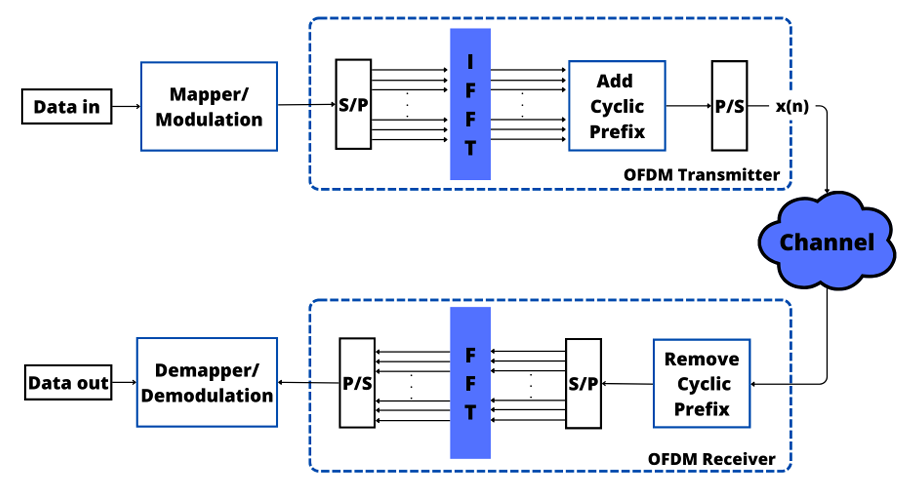
\includegraphics[width=0.70\linewidth]{Figures/01_ofdm_block_diagram.png}
    \caption{Block diagram of a baseband OFDM transmitter and receiver.
             The transmitter maps data onto $N$ subcarriers via an
             $N$-point IFFT, adds a cyclic prefix (CP), and transmits
             the time-domain signal.  The receiver removes the CP and
             applies an $N$-point FFT to recover the frequency-domain
             symbols.  Reproduced from~\cite{da2024survey}.}
    \label{fig:ofdm_block}
\end{figure}

\subsection{Subcarrier Structure and the IFFT/FFT Relationship}

Let the frequency-domain data symbol vector after constellation mapping be
\begin{equation}
    \bm{X} = \bigl[X_0,\; X_1,\; \dots,\; X_{N-1}\bigr]^T,
    \label{eq:freq_domain_vector}
\end{equation}
where $X_k$ is the complex symbol transmitted on the $k$-th subcarrier and
$N$ is the total number of subcarriers.  The time-domain OFDM signal is
obtained by applying the $N$-point IFFT~\cite{da2024survey,ali2016new}:
\begin{equation}
    x(n) = \frac{1}{\sqrt{N}} \sum_{k=0}^{N-1} X_k \, e^{\,j2\pi kn/N},
    \qquad n = 0,\, 1,\, \dots,\, N-1.
    \label{eq:ofdm_signal}
\end{equation}

\begin{keyinsight}
    The $1/\!\sqrt{N}$ normalization is a matter of convention.
    Some references use $1/N$ instead~\cite{ali2016new}.
    Throughout this document we adopt the $1/\!\sqrt{N}$ form
    so that the signal energy is preserved between the frequency and
    time domains (Parseval's theorem).
\end{keyinsight}

At the receiver, the frequency-domain symbols are recovered by the complementary
FFT operation:
\begin{equation}
    X_k = \frac{1}{\sqrt{N}} \sum_{n=0}^{N-1} x(n) \, e^{-\,j2\pi kn/N},
    \qquad k = 0,\, 1,\, \dots,\, N-1.
    \label{eq:fft_recovery}
\end{equation}

\subsection{Cyclic Prefix}

Before transmission, a \textbf{Cyclic Prefix (CP)} of length $N_{\mathrm{cp}}$
samples is prepended to each OFDM symbol by copying the last
$N_{\mathrm{cp}}$ samples of the IFFT output to the front.  The CP serves two
critical purposes~\cite{da2024survey}:
\begin{enumerate}
    \item \textbf{Inter-Symbol Interference (ISI) elimination:}
          As long as $N_{\mathrm{cp}}$ exceeds the maximum channel delay
          spread, the CP absorbs all multipath echoes from the previous symbol.
    \item \textbf{Circular convolution:}
          The CP converts the linear convolution with the channel into a
          circular convolution, enabling single-tap equalization in the
          frequency domain via the FFT.
\end{enumerate}

\subsection{Spectrum Efficiency: FDM vs.\ OFDM}

\begin{figure}[H]
    \centering
    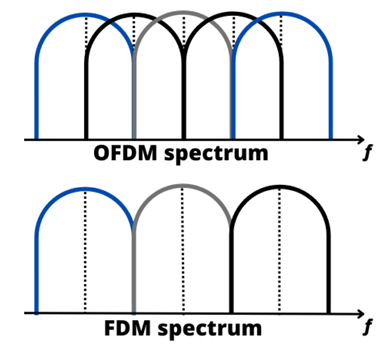
\includegraphics[width=0.45\linewidth]{Figures/02_fdm_vs_ofdm_spectrum.png}
    \caption{Ideal spectrum comparison between conventional Frequency-Division
             Multiplexing (FDM) and OFDM.  In FDM, guard bands between
             channels waste spectrum.  In OFDM, orthogonal subcarriers
             overlap without mutual interference, achieving significantly
             higher spectral efficiency.  Reproduced from~\cite{da2024survey}.}
    \label{fig:fdm_vs_ofdm}
\end{figure}

Figure~\ref{fig:fdm_vs_ofdm} illustrates why OFDM is spectrally superior:
the subcarriers are spaced at exactly $\Delta f = 1/T_s$ (where $T_s$ is the
useful symbol duration), ensuring orthogonality.  At every subcarrier's centre
frequency, all other subcarriers have a spectral null, so they contribute zero
interference~\cite{da2024survey}.


% ----------------------------------------------------------------------------
\section{PAPR: Definition and Significance}
\label{sec:papr_definition}
% ----------------------------------------------------------------------------

\subsection{Formal Definition}

Because the time-domain OFDM signal in \eqref{eq:ofdm_signal} is the sum of
$N$ independently modulated complex exponentials, the individual subcarrier
contributions can occasionally add up constructively, producing large amplitude
peaks.  The severity of this peaking is quantified by the
\textbf{Peak-to-Average Power Ratio (PAPR)}~\cite{da2024survey,ali2016new}:
\begin{equation}
    \mathrm{PAPR}\bigl(\bm{x}\bigr)
    = \frac{\displaystyle\max_{0 \le n \le N-1}\bigl|x(n)\bigr|^{2}}
           {E\Bigl[\bigl|x(n)\bigr|^{2}\Bigr]},
    \label{eq:papr_def}
\end{equation}
where the numerator is the peak instantaneous power and the denominator is the
average (expected) power of the OFDM symbol.

\begin{workingexample}[Numerical Feel for PAPR]
    For a 128-subcarrier OFDM system with QPSK modulation, the theoretical
    worst-case PAPR is $10\log_{10}(128) \approx 21.1$~dB---this occurs when
    all 128 subcarriers happen to align in phase at some instant $n$.
    In practice, such perfect alignment is extremely rare; the typical PAPR
    at a CCDF of $10^{-2}$ is around 10--12~dB~\cite{da2024survey}.
    Even so, this is far too high for efficient power amplifier operation.
\end{workingexample}

\subsection{CCDF as the Evaluation Metric}

Since PAPR is a random variable (it changes from one OFDM symbol to the next),
we characterise its statistical behaviour using the
\textbf{Complementary Cumulative Distribution Function (CCDF)}:
\begin{equation}
    \mathrm{CCDF}_{\mathrm{PAPR}}
    = \Pr\bigl(\mathrm{PAPR} > \mathrm{PAPR}_0\bigr),
    \label{eq:ccdf}
\end{equation}
where $\mathrm{PAPR}_0$ is a given threshold~\cite{da2024survey,zou2021novel}.
The CCDF tells us the probability that any randomly generated OFDM symbol will
exceed a certain PAPR level.  A good PAPR reduction technique shifts the CCDF
curve to the \emph{left}, meaning that high-PAPR events become much rarer.

For $N$ subcarriers with independent, identically distributed symbols and
Nyquist-rate sampling, the CCDF can be approximated
as~\cite{ali2016new}:
\begin{equation}
    \Pr\bigl(\mathrm{PAPR} \ge \mathrm{PAPR}_0\bigr)
    \approx 1 - \bigl(1 - e^{-\mathrm{PAPR}_0}\bigr)^{N}.
    \label{eq:ccdf_approx}
\end{equation}

\begin{figure}[H]
    \centering
    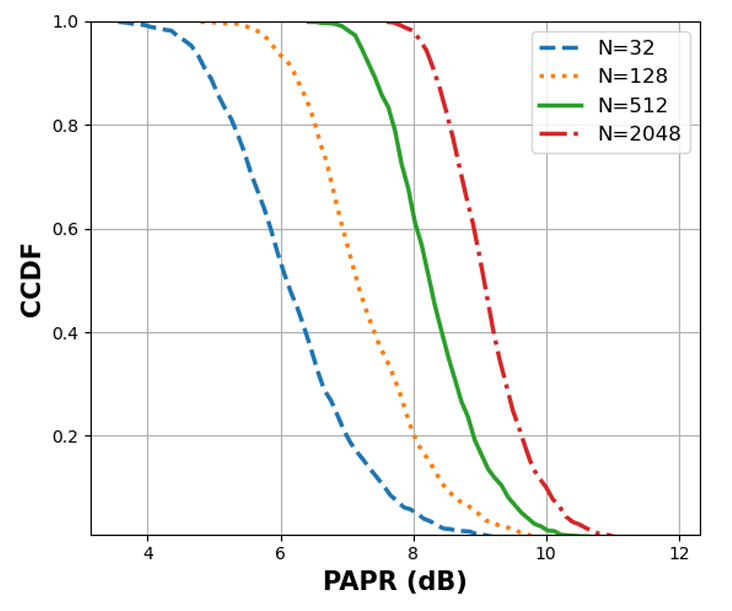
\includegraphics[width=0.55\linewidth]{Figures/03_ccdf_subcarriers.png}
    \caption{CCDF of PAPR for different numbers of subcarriers
             ($N = 32, 128, 512, 2048$) with 16-QAM modulation.
             As $N$ increases, the PAPR distribution shifts to the right,
             confirming that more subcarriers lead to higher PAPR.
             Reproduced from~\cite{da2024survey}.}
    \label{fig:ccdf_subcarriers}
\end{figure}

\subsection{The HPA Nonlinearity Problem}

Why does high PAPR matter in practice?  The answer lies in the
\textbf{High-Power Amplifier (HPA)} at the transmitter.
An ideal HPA would amplify any input linearly, regardless of amplitude.
In reality, every power amplifier has a \emph{saturation region}:
when the input signal exceeds a certain amplitude, the output clips
or compresses, introducing severe nonlinear distortion~\cite{da2024survey}.

To avoid entering this nonlinear zone, the HPA must operate with sufficient
\textbf{Input Back-Off (IBO)}:
\begin{equation}
    \mathrm{IBO\;(dB)} = 10\log_{10}\!\left(\frac{P_{\mathrm{sat}}}{P_{\mathrm{avg}}}\right),
    \label{eq:ibo}
\end{equation}
where $P_{\mathrm{sat}}$ is the amplifier's saturation power and
$P_{\mathrm{avg}}$ is the average input signal power.  For an OFDM signal
with $\mathrm{PAPR} = 12$~dB, the IBO must be at least 12~dB, meaning
the amplifier operates far below its maximum capacity most of the time.
This directly costs \emph{power efficiency} and \emph{hardware complexity}
in real systems~\cite{da2024survey}.

\begin{keyinsight}
    Reducing PAPR by even 3--4~dB translates to a significant improvement
    in HPA efficiency, reduced heat dissipation, longer battery life in
    mobile devices, and lower deployment costs.  This is why PAPR reduction
    is one of the most active research areas in OFDM system
    design~\cite{da2024survey}.
\end{keyinsight}


% ----------------------------------------------------------------------------
\section{Classical PAPR Reduction Techniques --- A Brief Survey}
\label{sec:classical_techniques}
% ----------------------------------------------------------------------------

Before diving into SLM, it is helpful to briefly survey the landscape of
classical PAPR reduction techniques, as many of them appear as baselines
in the ML-enhanced approaches studied later.  These can be broadly
classified into \textbf{signal distortion} techniques and
\textbf{signal scrambling} (or probabilistic) methods~\cite{da2024survey}.

\subsection{Signal Distortion Techniques}

\paragraph{Clipping and Filtering.}
The simplest approach: any signal sample exceeding a threshold $A$ is
clipped to that threshold.  Filtering is then applied to suppress
out-of-band spectral regrowth.  The clipped signal is~\cite{zou2021novel}:
\begin{equation}
    x'(n) =
    \begin{cases}
        x(n), & |x(n)| \le A, \\[4pt]
        \dfrac{A}{|x(n)|}\, x(n), & |x(n)| > A,
    \end{cases}
    \label{eq:clipping}
\end{equation}
where $A = \mathrm{CR}\cdot\sqrt{P_{\mathrm{avg}}}$ and $\mathrm{CR}$ is
the clipping ratio~\cite{zou2021novel}.

\begin{figure}[H]
    \centering
    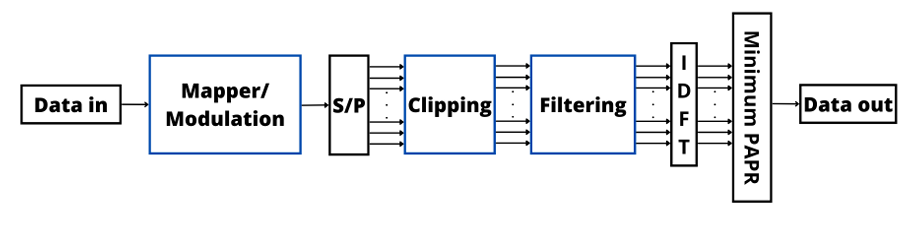
\includegraphics[width=0.75\linewidth]{Figures/04_clipping_filtering.png}
    \caption{Block diagram of an OFDM transmitter with clipping and filtering.
             The signal is clipped in the time domain, then filtered in the
             frequency domain to remove out-of-band distortion.
             Reproduced from~\cite{da2024survey}.}
    \label{fig:clipping_filtering}
\end{figure}

\textbf{Pros:} Simple, no side information needed.
\textbf{Cons:} Introduces in-band distortion (increased BER) and
out-of-band radiation~\cite{da2024survey}.

\paragraph{Active Constellation Extension (ACE).}
Extends outer constellation points away from the decision boundaries
to reduce peak power, without affecting the BER.  No side information
is required~\cite{da2024survey}.

\begin{figure}[H]
    \centering
    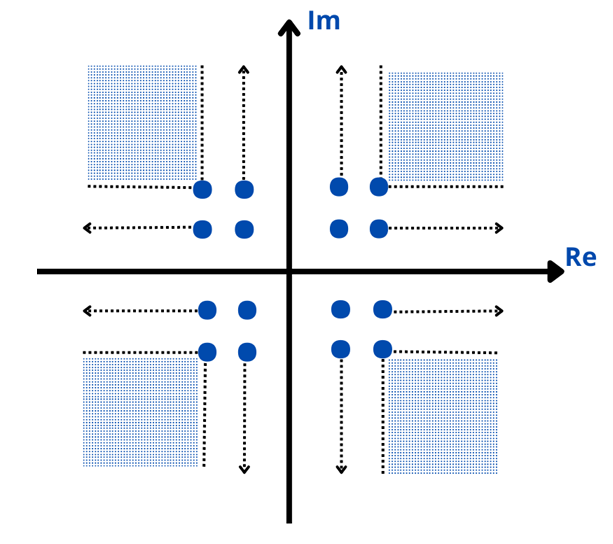
\includegraphics[width=0.55\linewidth]{Figures/05_ace_constellation.png}
    \caption{Active Constellation Extension for 16-QAM.
             Outer constellation points are extended into ``feasible regions''
             (shaded), reducing the PAPR without crossing decision boundaries.
             Reproduced from~\cite{da2024survey}.}
    \label{fig:ace}
\end{figure}

\subsection{Signal Scrambling Methods}

These methods alter the signal representation \emph{without distortion} to
find a low-PAPR version.

\paragraph{Partial Transmit Sequence (PTS).}
The input data block is partitioned into $V$ disjoint sub-blocks, each
transformed by an IFFT independently.  The sub-blocks are then weighted by
phase factors $b_v \in \{e^{j\phi} : \phi \in \Phi\}$ and summed.
The phase combination yielding the lowest PAPR is selected for
transmission~\cite{da2024survey}.

\begin{figure}[H]
    \centering
    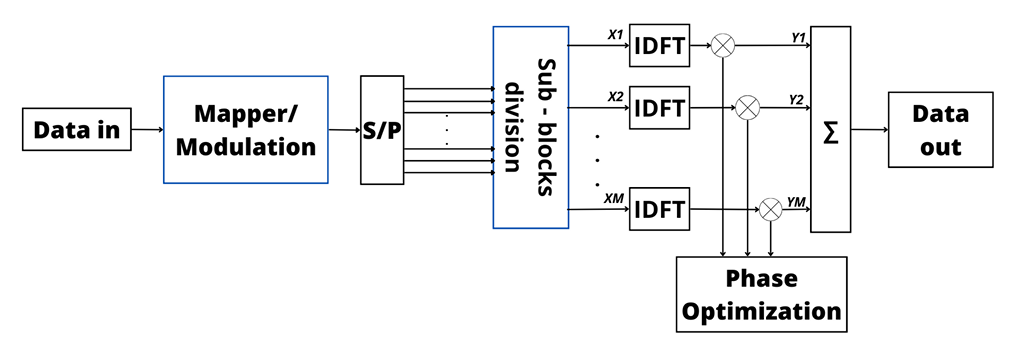
\includegraphics[width=0.85\linewidth]{Figures/06_pts_block_diagram.png}
    \caption{Block diagram of an OFDM transmitter with Partial Transmit
             Sequence (PTS).  The data is split into $V$ sub-blocks,
             each weighted by a phase factor after the IDFT.
             The combination with the lowest PAPR is transmitted.
             Reproduced from~\cite{da2024survey}.}
    \label{fig:pts}
\end{figure}

\paragraph{Tone Reservation (TR) and Tone Injection (TI).}
TR reserves a set of subcarriers exclusively for peak-cancelling signals,
while TI adds carefully designed tones to the data subcarriers.  Both reduce
PAPR without distorting data symbols, but at the cost of reduced spectral
efficiency (TR) or increased average power (TI)~\cite{da2024survey}.

\paragraph{Interleaving.}
Multiple interleaving patterns are applied to the data, and the pattern
producing the lowest PAPR is selected, similar to SLM but using
permutation rather than phase rotation~\cite{da2024survey}.

Table~\ref{tab:classical_comparison} summarizes the key trade-offs.

\begin{table}[H]
    \centering
    \caption{Comparison of classical PAPR reduction techniques.  Data adapted
             from~\cite{da2024survey}.}
    \label{tab:classical_comparison}
    \begin{tabular}{@{} l c c c c @{}}
        \toprule
        \textbf{Technique} & \textbf{BER Impact} & \textbf{Complexity} & \textbf{Side Info} & \textbf{Distortion} \\
        \midrule
        PTS          & None  & High     & Yes & No  \\
        SLM          & None  & High     & Yes & No  \\
        Interleaving & None  & Low      & Yes & No  \\
        Clipping     & Yes   & Low      & No  & Yes \\
        TI           & None  & High     & No  & No  \\
        TR           & None  & High     & Yes & No  \\
        ACE          & None  & Moderate & No  & No  \\
        \bottomrule
    \end{tabular}
\end{table}


% ----------------------------------------------------------------------------
\section{The SLM Algorithm --- Formal Review}
\label{sec:slm_algorithm}
% ----------------------------------------------------------------------------

Among all classical PAPR reduction techniques, \textbf{Selected Mapping (SLM)}
stands out for its combination of distortion-free operation and applicability
to any modulation format and any number of subcarriers~\cite{ali2016new,da2024survey}.
This section gives a complete, self-contained review.

\begin{figure}[H]
    \centering
    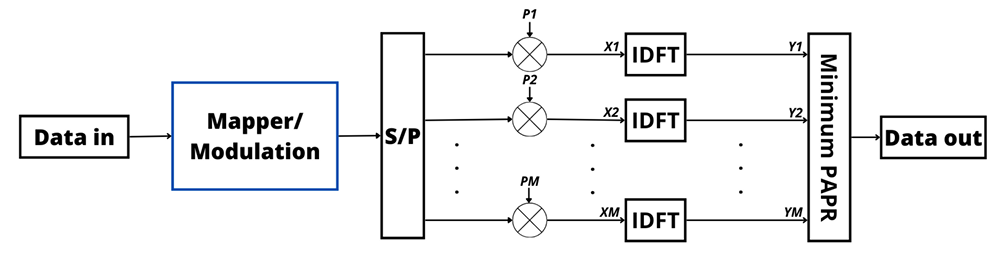
\includegraphics[width=0.75\linewidth]{Figures/07_slm_block_diagram.png}
    \caption{Block diagram of an OFDM transmitter with Selected Mapping (SLM).
             $U$ different phase sequences are applied to the frequency-domain
             data \emph{before} the IDFT.  The candidate signal with the lowest
             PAPR is selected for transmission.
             Reproduced from~\cite{da2024survey}.}
    \label{fig:slm_block}
\end{figure}

\subsection{Phase Sequence Generation and Design}

The core idea of SLM is to generate $U$ alternative representations of the
same data block by multiplying the frequency-domain symbols with $U$ different
\textbf{phase sequences}.  Let the $u$-th phase sequence be~\cite{ali2016new}:
\begin{equation}
    \bm{\psi}_u = \bigl[\psi_{u,0},\;\psi_{u,1},\;\dots,\;\psi_{u,N-1}\bigr]^T,
    \qquad u = 1,\,2,\,\dots,\,U,
    \label{eq:phase_sequence}
\end{equation}
where each element is a unit-magnitude complex number:
\begin{equation}
    \psi_{u,k} = e^{\,j\varphi_{u,k}},
    \qquad \varphi_{u,k} \in [0,\;2\pi).
    \label{eq:phase_element}
\end{equation}
In the simplest case, $\varphi_{u,k}$ is drawn uniformly at random
from $[0,2\pi)$~\cite{ali2016new}.  In practice, the phase alphabet is often
restricted to a finite set such as $\{+1,\,-1,\,+j,\,-j\}$
(i.e., $\varphi_{u,k} \in \{0,\, \pi/2,\, \pi,\, 3\pi/2\}$)
to reduce implementation complexity~\cite{ali2016new}.

\begin{keyinsight}
    One of the $U$ sequences is always set to the all-ones vector
    $\bm{\psi}_1 = [1,\,1,\,\dots,\,1]^T$, so that one candidate is the
    unmodified original signal.  This guarantees that SLM can never
    \emph{increase} the PAPR beyond the original value~\cite{ali2016new}.
\end{keyinsight}

\subsection{Candidate Signal Generation}

Each phase sequence is applied element-wise (Hadamard product) to the
frequency-domain data vector~\cite{ali2016new}:
\begin{equation}
    \bm{X}_u = \bm{X} \odot \bm{\psi}_u,
    \qquad u = 1,\,2,\,\dots,\,U.
    \label{eq:slm_candidates_freq}
\end{equation}
The corresponding time-domain candidate signals are then obtained via the
IFFT~\cite{ali2016new}:
\begin{equation}
    \bm{x}_u = \mathrm{IFFT}\{\bm{X}_u\}
             = \mathrm{IFFT}\{\bm{X} \odot \bm{\psi}_u\},
    \qquad u = 1,\,2,\,\dots,\,U.
    \label{eq:slm_candidates_time}
\end{equation}

\subsection{PAPR Evaluation and Candidate Selection}

The PAPR of each candidate is computed, and the one with the
\emph{minimum} PAPR is selected for transmission~\cite{ali2016new}:
\begin{equation}
    \hat{u} = \arg\min_{1 \le u \le U}\;
    \mathrm{PAPR}\bigl(\bm{x}_u\bigr).
    \label{eq:slm_selection}
\end{equation}
The transmitted signal is then $\bm{x}_{\hat{u}}$.

\subsection{Side Information (SI)}

The receiver needs to know \emph{which} phase sequence was used, so it can
reverse the phase rotation and recover the original data:
\begin{equation}
    \hat{\bm{X}} = \bm{X}_{\hat{u}} \odot \bm{\psi}_{\hat{u}}^{*},
    \label{eq:slm_recovery}
\end{equation}
where $(\cdot)^{*}$ denotes the element-wise complex conjugate
(since $|\psi_{u,k}|=1$, dividing by $\psi_{u,k}$ is the same as multiplying
by $\psi_{u,k}^{*}$).

The index $\hat{u}$ is the \textbf{side information (SI)}, which requires
$\lceil\log_2 U\rceil$ bits per OFDM symbol.  For example,
$U=16$ candidates require 4 SI bits~\cite{ali2016new,da2024survey}.

\begin{misconception}
    \textbf{``Side information is a minor overhead.''} \\
    While $\lceil\log_2 U\rceil$ bits may seem negligible, these bits must be
    received \emph{error-free} for the receiver to undo the correct phase
    rotation.  If even one SI bit is received in error, the \emph{entire}
    OFDM symbol is incorrectly de-rotated, causing a burst of bit errors.
    Protecting SI typically requires additional channel coding or embedding
    schemes, which add further complexity and overhead~\cite{da2024survey}.
\end{misconception}


% ----------------------------------------------------------------------------
\section{Worked Numerical Recap}
\label{sec:worked_example}
% ----------------------------------------------------------------------------

\begin{workingexample}[SLM with $N=8$, $U=4$]
Consider a toy OFDM system with $N=8$ subcarriers and QPSK modulation.
The frequency-domain data vector is:
\[
    \bm{X} = [1+j,\; -1+j,\; 1-j,\; -1-j,\; 1+j,\; -1+j,\; 1-j,\; -1-j]^T.
\]
We use $U=4$ phase sequences with alphabet $\{+1,-1\}$:
\begin{align*}
    \bm{\psi}_1 &= [+1,\,+1,\,+1,\,+1,\,+1,\,+1,\,+1,\,+1]^T & \text{(identity)}, \\
    \bm{\psi}_2 &= [+1,\,-1,\,+1,\,-1,\,+1,\,-1,\,+1,\,-1]^T, \\
    \bm{\psi}_3 &= [+1,\,+1,\,-1,\,-1,\,+1,\,+1,\,-1,\,-1]^T, \\
    \bm{\psi}_4 &= [+1,\,-1,\,-1,\,+1,\,+1,\,-1,\,-1,\,+1]^T.
\end{align*}

\textbf{Step 1: Generate candidates.}
For each $u$, compute $\bm{X}_u = \bm{X} \odot \bm{\psi}_u$,
then $\bm{x}_u = \mathrm{IFFT}\{\bm{X}_u\}$.

\textbf{Step 2: Compute PAPR.}
Evaluate $\mathrm{PAPR}(\bm{x}_u)$ for $u = 1,\dots,4$.

\textbf{Step 3: Select.}
Suppose the PAPR values are 9.2~dB, 6.1~dB, 7.8~dB, and 5.3~dB for
$u = 1,2,3,4$ respectively.  We select $\hat{u}=4$ (lowest PAPR = 5.3~dB).

\textbf{Step 4: Transmit.}
Send $\bm{x}_4$ along with 2 bits of SI ($\hat{u}=4 \to$ binary ``11'').

\textbf{Step 5: Recover.}
The receiver uses the SI to look up $\bm{\psi}_4$ and computes
$\hat{\bm{X}} = \bm{X}_4 \odot \bm{\psi}_4^{*}$ to recover
the original $\bm{X}$.

In this example, SLM reduced the PAPR from 9.2~dB (original) to 5.3~dB---a
gain of 3.9~dB---at the cost of 4 IFFT operations and 2 SI bits.
\end{workingexample}


% ----------------------------------------------------------------------------
\section{SLM Variants Overview}
\label{sec:slm_variants}
% ----------------------------------------------------------------------------

Several variants of classical SLM appear as baselines or building blocks in
the ML-enhanced approaches studied in later chapters:

\begin{itemize}
    \item \textbf{Conventional SLM}~\cite{ali2016new}:
          Uses random or pseudo-random phase sequences with a finite phase
          alphabet.  The PAPR reduction increases with $U$ but with
          diminishing returns (see Figure~\ref{fig:slm_ccdf_varying_m}).

    \item \textbf{Modified SLM}~\cite{da2024survey}:
          Reduces the number of IFFT operations required by exploiting
          structural relationships between phase sequences.

    \item \textbf{Extended SLM (ESLM)}~\cite{hao2019extended}:
          Extends SLM by allowing phase factors to take
          \emph{any} value in $[0,2\pi)$ (rather than a discrete alphabet),
          and determines them adaptively through neural network training.
          This is one of the ML-enhanced approaches covered in
          Chapter~\ref{ch:eslm_ae}.

    \item \textbf{GA-Optimized SLM}~\cite{ali2016new}:
          Uses a Genetic Algorithm to search for the optimal phase
          rotation factors instead of exhaustive or random search.
          This is covered in Chapter~\ref{ch:ga_slm}.
\end{itemize}

\begin{figure}[H]
    \centering
    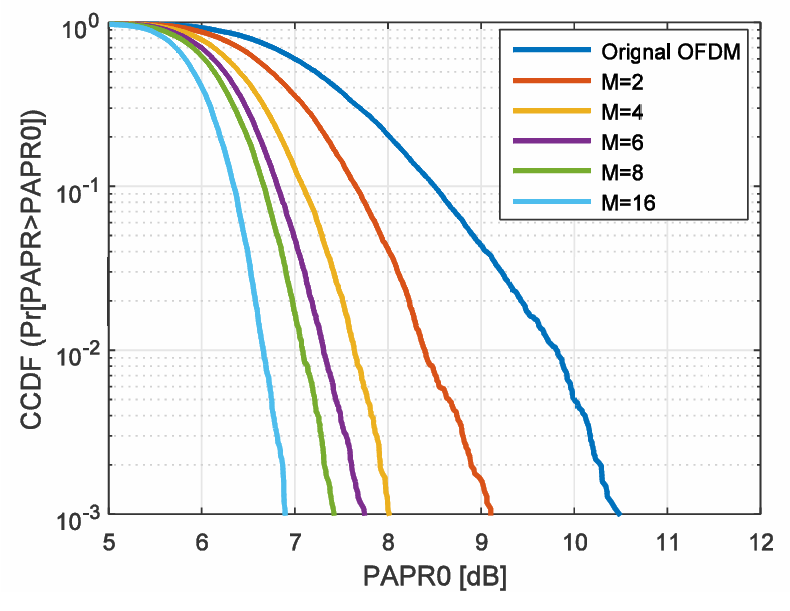
\includegraphics[width=0.55\linewidth]{Figures/08_slm_ccdf_varying_m.png}
    \caption{CCDF of PAPR for conventional SLM with different numbers of
             phase sequences $U$ ($N=128$, QPSK).
             Increasing $U$ improves PAPR but with diminishing returns:
             the gap between $U=8$ and $U=16$ is only about 0.5~dB.
             Reproduced from~\cite{ali2016new}.}
    \label{fig:slm_ccdf_varying_m}
\end{figure}


% ----------------------------------------------------------------------------
\section{The Three Core Limitations of Classical SLM}
\label{sec:slm_limitations}
% ----------------------------------------------------------------------------

Despite its elegance, classical SLM suffers from three fundamental limitations
that motivate the ML-enhanced approaches explored in subsequent chapters.

\subsection{Limitation 1: Computational Complexity}

Each OFDM symbol requires $U$ full $N$-point IFFT operations---one per
candidate.  The complexity of a single $N$-point IFFT is
$\mathcal{O}(N\log_2 N)$, so the total SLM complexity per symbol
is~\cite{ali2016new,da2024survey}:
\begin{equation}
    \mathcal{C}_{\mathrm{SLM}} = \mathcal{O}\bigl(U \cdot N\log_2 N\bigr).
    \label{eq:slm_complexity}
\end{equation}

\begin{workingexample}[Complexity Numbers]
    For a 5G NR-like system with $N=2048$ subcarriers and $U=16$ candidates,
    each OFDM symbol requires $16 \times 2048 \times \log_2(2048)
    = 16 \times 2048 \times 11 = 360{,}448$ complex multiply-accumulate
    operations just for the PAPR reduction step.  At a symbol rate of
    14 symbols per slot $\times$ 2000 slots/s $= 28{,}000$ symbols/s,
    this amounts to over 10 billion operations per second---a non-trivial
    computational burden for real-time implementation.
\end{workingexample}

\subsection{Limitation 2: Side Information Overhead}

The $\lceil\log_2 U\rceil$ SI bits per symbol carry a dual cost:
\begin{enumerate}
    \item \textbf{Bandwidth:} They consume subcarriers (or dedicated
          signaling) that could otherwise carry user data, reducing
          spectral efficiency.
    \item \textbf{Reliability:} An error in the SI bits causes \emph{all}
          data bits in the symbol to be decoded incorrectly.
          Therefore, SI bits typically need stronger error protection
          than regular data, adding further overhead~\cite{da2024survey}.
\end{enumerate}

\subsection{Limitation 3: Blind Detection Difficulty}

To avoid the SI overhead entirely, one could attempt \textbf{blind detection}:
the receiver tries all $U$ phase sequences and determines the correct one
without explicit SI.  However:
\begin{itemize}
    \item The receiver must perform $U$ full FFT operations per symbol.
    \item Decision metrics (e.g., based on pilot symbols or higher-order
          statistics) are unreliable at low SNR.
    \item The probability of choosing the wrong phase sequence is
          non-negligible, especially for large $U$~\cite{da2024survey}.
\end{itemize}

Blind SLM detection is therefore an \emph{open problem} particularly
well-suited to ML-based solutions, which can learn complex statistical
patterns that classical detectors cannot capture.


% ----------------------------------------------------------------------------
\section{Transition: From Classical Limitations to ML Solutions}
\label{sec:transition}
% ----------------------------------------------------------------------------

The three limitations of classical SLM map directly to three categories of
ML-enhanced solutions explored in the following chapters:

\begin{enumerate}
    \item \textbf{Complexity reduction} $\longrightarrow$
          Neural networks can learn to produce low-PAPR signals in a
          \emph{single forward pass}, replacing the $U$ IFFT operations
          with a fixed-complexity inference step
          (Chapters~\ref{ch:prnet},~\ref{ch:nn_scf},~\ref{ch:eslm_ae},~\ref{ch:prdun},~\ref{ch:dl_ae_optical}).

    \item \textbf{Side information elimination} $\longrightarrow$
          Autoencoders that jointly learn encoding and decoding can
          embed the phase selection implicitly, removing the need for
          explicit SI transmission
          (Chapters~\ref{ch:prnet},~\ref{ch:eslm_ae},~\ref{ch:dl_ae_optical}).

    \item \textbf{Intelligent search} $\longrightarrow$
          Evolutionary algorithms (e.g., Genetic Algorithms) and
          model-driven unfolding networks can navigate the vast
          phase-sequence search space far more efficiently than
          exhaustive or random search
          (Chapters~\ref{ch:ga_slm},~\ref{ch:prdun}).
\end{enumerate}

\begin{keyinsight}
    No single ML approach solves all three limitations simultaneously.
    Each technique in the following chapters addresses a different subset
    of these challenges, with its own set of trade-offs.  The comparative
    analysis in Chapter~\ref{ch:comparative} will map these trade-offs
    explicitly.
\end{keyinsight}
